\begin{table*}[h]
    \caption{\footnotesize Summary of the task groups used by \ours{}. }
    \label{tab:environment_summary}
    \centering
    \resizebox{\textwidth}{!}{%
        \begin{tabular}{c|c c c c c}
        \toprule
            Task Group & \# Train Tasks & \# Test Tasks & Maximum Turns & Env Feedback & Uses COT \\
            \midrule
             Twenty questions & 1499 & 367 & 20 & LLM generated & \ding{55} \\
             Guess my city & 500 & 185 & 20 & LLM generated & \ding{55} \\
             Wordle & 1515 & 800 & 6 & Hardcoded program & \checkmark \\
             Cellular automata & 1000 & 500 & 6 & Hardcoded program & \checkmark \\
             Customer service & 628 & 200 & 20 & LLM generated & \ding{55} \\
             Murder mystery & 203 & 50 & 20 & LLM generated & \ding{55} \\
             Mastermind & 1000 & 500 & 12 & Hardcoded program & \checkmark \\
             Battleship & 1000 & 200 & 20 & Hardcoded program & \checkmark \\
             Minesweeper & 1000 & 200 & 20 & Hardcoded program & \checkmark \\
             Bandit best arm selection & 81 & 1 & 21 & Hardcoded program & \checkmark \\
             \bottomrule
        \end{tabular}
    }
    \vspace{-0.3cm}
\end{table*}

\section{\ours{}}

The goal of our paper is to develop a scalable method to instill better strategic exploration and sequential decision-making capabilities into LLMs. Prior works~\citep{krishnamurthy2024largelanguagemodelsexplore} have shown that LLMs can perform poorly on even the simple decision making task of multi-armed bandits. \citet{nie2024evolveevaluatingoptimizingllms} has since then demonstrated that LLMs can be taught to perform better on bandits after fine-tuning them on synthetic trajectories generated by known algorithms such as UCB. However, this idea is limited in scope for three reasons: \textbf{(1)} we want LLMs to perform strategic exploration and decision making in more complex settings, \textbf{(2)} for most tasks, there is no known algorithm like UCB to generate good synthetic trajectories from, \textbf{(3)} it can be infeasible to collect data for all tasks that we care about.

We aim to solve these issues using our method, \ours{}. First, we design a suite of complex decision-making tasks that require strategic information gathering to succeed. Next, we show that in the absence of known good algorithms, existing LLMs can generate trajectories with better decision making behaviors through diversity-encouraging sampling. We then finetune the LLMs to prefer higher performing trajectories (in a fashion similar to STaR~\citep{zelikman2022starbootstrappingreasoningreasoning}) and show that this leads to better decision making abilities at test-time. More importantly, these behaviors often generalize to unseen task groups without additional training. Finally, we propose a general curriculum learning algorithm that can dynamically choose which subset of tasks to train on next to improve data efficiency of such training methods. We next describe each component of \ours{}.


\subsection{Task Design}


The first component of \ours{} is to design a set of task groups that we can evaluate and train LLMs on. The task groups we want should have the following desired properties: \textbf{(1)} they are purely text based, \textbf{(2)} they require multi-turn interaction, where the agents have to both understand prior history in its context and choose actions that maximize the probability of success in the future, \textbf{(3)} they are partially observable, i.e., the observations do not capture the full state or hidden information, so the agents must simultaneously explore to reveal more information and exploit to solve the task efficiently, \textbf{(4)} they are diverse and require different strategies to succeed. 


With these requirements in mind, we design 10 task groups in our paper. On all of them, we employ an LLM as the agent that is given a task it needs to solve through sequential interaction with the task-specific environment, which provides both observations for intermediate timesteps given the agent's actions and also a task reward at the end of an episode. 
For tasks requiring general knowledge about the world to generate intermediate observations, we employ another LLM (typically GPT-4o-mini) as the environment. For tasks that have rule-based observations and rewards, we find that using hardcoded programs as the verifier/observation generator is more reliable than LLMs, similar to~\citet{deepseekai2025deepseekr1incentivizingreasoningcapability}. In order to prevent reward hacking, we also use either another LLM or a hardcoded program as a judge to filter out unsuccessful trajectories that got incorrectly labeled as successful by the task environment (see \cref{section:environment_hacking} for more on environment hacking). We also find that for task groups requiring complex reasoning, letting the agent think using chain-of-thought (COT) prompting~\citep{wei2022chain, kojima2022large} before generating a final answer improves its performance significantly, similar to ReAct~\citep{yao2023reactsynergizingreasoningacting}. We provide a brief description of our task groups here, please refer to \cref{tab:environment_summary} for their summary and \cref{section:appendix_environment_design} for more details.

Following prior work~\citep{abdulhai2023lmrl}, we include classic guessing games like \textit{twenty questions} and \textit{guess my city} in our list of task groups. They require guessing a secret topic as quickly as possible by asking a sequence of questions and observing the answers. We also employ \textit{Wordle} and \textit{Mastermind}, where the agent needs to guess a secret 5-letter word and 4-digit code respectively. The environments for these task groups provide feedback in terms of similarity between the guess and the target word/code, and the agent needs to refine their guesses in future turns to maximize information gathering. We design \textit{customer service} and \textit{murder mystery} as dynamic text-based task groups: an LLM plays the role of the task environment, which is provided with the criterion for task success and generates dynamic intermediate observations based on this criterion. 

A desirable capability in LLMs is to code and refine based on interpreter feedback. To simulate this process with a toy case, we design \textit{Cellular Automata}, where the agent needs to make inferences about the transition rule in 1D elementary cellular automata~\citep{wolfram1983statistical, cook2004universality} by observing inputs and outputs. The agent receives the outputs generated from their predicted transition rule and they have to refine their predictions based on it. Next, we incorporate \textit{Minesweeper} and \textit{Battleship} based on classical games, which require the agent to interact with 2D grids to find hidden items within a fixed number of turns and refine their guesses based on per-turn observations. 

Finally, we incorporate a modified version of the multi-armed bandit~\citep{slivkins2024introductionmultiarmedbandits} task group from prior works~\citep{krishnamurthy2024largelanguagemodelsexplore,nie2024evolveevaluatingoptimizingllms} with the following distinctions: \textbf{(1)} we let the agent employ chain-of-thought reasoning before choosing arms so that they can transfer good strategies learned from other tasks, \textbf{(2)} we let the agent interact with the task environment in a multiturn way, \textbf{(3)} instead of reducing regret, we work on the bandit best arm selection~\citep{audibert:hal-00654404,wang2024bestarmidentificationfixed} problem, where we let the agent choose arms and observe rewards for a fixed number of turns and then measure its accuracy in deciding the arm with the highest reward. This is done to reduce computational cost over generating COTs for a large number of turns, since the difference in regret between different models is not meaningful when the number of turns is not large enough.

\subsection{Dataset construction}

In order to learn from these task groups, we must first generate data from them. It is crucial that the data we generate are diverse which would allow the model to learn different strategies without the risk of overfitting. We accomplish this by generating a large number of trajectories at a high temperature with Min-p sampling~\citep{nguyen2024turning}. Min-p sampling works by using an adaptive threshold $p_\text{scaled} \propto p_\text{max}$, where $p_\text{max}$ is the highest probability predicted by the model on the next token, to truncate the vocabulary to tokens that have a probability larger than $p_\text{scaled}$ and sample from them --- this enables us to generate diverse yet coherent trajectories at a higher temperature. We note that training data generation for \ours{} could be improved by adopting more advanced methods for guiding exploration such as ~\citet{murty2024bagel,yang2024react}; however, we opt for sampling with high temperature for its simplicity and leave these other options for future work.


For each task in a set of chosen tasks (e.g., uniformly sampled), we generate $n_\text{sample}$ trajectories and then construct a preference pair $(h_{w}, h_{l})$ where $h_{w}$ is the highest scoring trajectory (trajectory that succeeds and does so at the fewest number of turns) and $h_{l}$ is randomly sampled from the lower scoring (failed  or takes substantially more turns to succeed) trajectories. We choose $h_l$ randomly instead of choosing the worst one to increase the diversity of our dataset. We treat $h_w$ and $h_l$ as proxies for desirable and undesirable behaviors. A dataset $\mathcal{D} = \left\{\left(h^{w}, h^{l}\right)^{(i)}\right\}_{i=1}^N$ is a collection of such trajectory pairs.

\subsection{Optimization}
\label{sec:opt}

\paragraph{Supervised fine-tuning.} If we take the winning episodes as the expert behavior, then we can discard the losing episode and maximize the likelihood of winning episodes:

\begin{align}
    \mathcal{L}_\text{SFT}(\mathcal{D}_\text{SFT}) = -\mathbb{E}_{\mathcal{D}_\text{SFT}} \left[ \frac{1}{\sum_{t=0}^{|h_w|}|a_t^w|}\sum_{t=0}^{|h_w|} \log \pi_\theta \left(a^w_t \mid h^w_{:t}\right) \right]
\end{align}
where $\mathcal{D}_\text{SFT}$ is the dataset used for supervised fine-tuning and $|a|$ is the number of tokens for the agent response (discarding the environment generation). This is akin to rejection sampling fine-tuning~\citep{gulcehre2023reinforcedselftrainingrestlanguage,dong2023raft,mukobi2023superhfsupervisediterativelearning} seen in prior work.

\paragraph{Direct preference optimization.} A popular approach for finetuning LLMs is DPO~\citep{rafailov2024direct} where one directly optimizes the Bradley-Terry model~\citep{bradley1952rank} for preferences. In our setting, each trajectory consists of multiple rounds of interactions so the original DPO objective does not apply. We instead use a multi-turn version of DPO introduced in ~\citet{rafailov2024rqlanguagemodel}:
\begin{multline}
    \mathcal{L}_\text{DPO}(\gD_\text{DPO}) = -\E_{\gD_\text{DPO}}\Bigg[\log \sigma\Bigg( 
    \sum_{t=0}^{|h^w|}\beta \log\frac{\pi_\theta(a_t^w \mid h_{:t}^w)}{\pi_\text{ref}(a_t^w \mid h_{:t}^w)} \\
    - \sum_{t=0}^{|h^l|}\beta \log\frac{\pi_\theta(a_t^l \mid h_{:t}^l)}{\pi_\text{ref}(a_t^l \mid h_{:t}^l)}
    \Bigg)\Bigg]
\end{multline}

where $\gD_\text{DPO}$ is the preference dataset, $a_t^w$ and $a_t^l$ are the action tokens generated by the model at turn $t$ in the preferred and dispreferred trajectories, $h^w$ and $h^l$, respectively.
$\pi_\text{ref}$ is the reference policy, for which we use the initial model.
The main difference with standard DPO here is that we only calculate the loss on the action tokens --- the log probability ratios of the environment generated tokens are not included in the loss.

We note that we use DPO because it is less compute intensive. DPO allows us to decouple the data collection and policy improvement steps and offload them on different machines. However, in principle, one could also employ online RL with more resources. Following prior work that shows the efficacy of online RL compared to offline algorithms~\citep{xu2024dposuperiorppollm,tajwar2024preferencefinetuningllmsleverage}, we expect doing \ours{} with online RL would lead to even stronger results.

\paragraph{Combining objectives.} 

Finally, prior works have noted DPO having the unintended effect of reducing the probability of preferred trajectories as well, known as unintentional unalignment~\citep{razin2024unintentionalunalignmentlikelihooddisplacement}, which can affect model performance. The RPO objective~\citep{pang2024iterativereasoningpreferenceoptimization}, by combining SFT and DPO loss, has shown promising results in mitigating this issue. Formally, the RPO loss is:

\begin{equation} \label{eq:rpo_formula}
    \mathcal{L}_{\text{RPO}}(\mathcal{D}_\text{DPO}) = \mathcal{L}_\text{DPO}(\gD_\text{DPO}) + \alpha \mathcal{L}_\text{SFT}(\gD_\text{DPO})
\end{equation}

where $\alpha$ is a hyper-parameter. Following ~\citet{pang2024iterativereasoningpreferenceoptimization}, we set $\alpha$ to be 1.0 for the rest of this paper.


\subsection{Scalable Online Curriculum Learning} \label{section:curriculum}
The core idea of \ours{} is to fine-tune the model on a large number of decision making problems to acquire general decision making ability. It is relatively easy to design a large number of tasks, but it is harder to decide which task to train on. A major obstacle is that different tasks may have a large range of difficulty. Unlike pretraining where the model can generally make progress on any given sample (i.e., decrease next-token prediction loss), an RL agent cannot make meaningful progress without collecting good experience. As such, if a task is too difficult for the current model, the model would not generate trajectories with meaningful learning signals. Since generating a trajectory is expensive, it stands to reason that we want to prioritize the tasks where the model can make meaningful progress, which is a form of curriculum learning~\citep{bengio2009curriculum}.

Without additional assumptions, the only way to know whether a task would yield good learning signals is to actually perform a rollout in that task, which is expensive.
In fact, in this particular scenario, the major cost for training is actually data generation rather than model updates.
As such, this naive approach would not save us time or computation.
A desideratum for an efficient curriculum is the ability to know whether certain tasks will yield data with learning signals without actually performing the rollout.
A natural assumption is that similar tasks would have similar levels of learning signal. 
These groupings can be obtained through meta data or prior knowledge.\footnote{While this requirement may seem restrictive, we believe assumptions of similar effects are likely needed for any form of curriculum learning to be computationally efficient.}

\paragraph{Measuring learning potential.} We will use $h \sim \pi \circ \tau$ to denote sampling one episode from the task $\tau$ using the policy $\pi$. The average performance of $\pi$ on $\tau$ is $R_\pi(\tau) = \E_{h \sim \pi \circ \tau }\left[r(h)\right]$ and the variance is $\sigma^2_\pi(\tau) = \E_{h \sim \pi \circ \tau }\left[(r(h) - R_\pi(\tau))^2\right]$. Based on these, we can define:
\begin{align}
\label{eq:nu}
    \nu_\pi(\tau) = \frac{\sqrt{\sigma^2_\pi(\tau)}}{R_\pi(\tau)}.
\end{align}
This quantity is known as the coefficient of variation in statistics, a dimensionless quantity that measures the population's variability relative to the mean. 

We argue that this quantity is an ideal measure of the learning potential for a single task. DPO requires a pair of positive and negative samples~\footnote{We hypothesize this quantity would also apply to online RL since if all sampled trajectories have the same reward the policy gradient update would be $0$.}. Intuitively, the pair should be sufficiently different so the model can tell the two apart --- for example, prior work~\citep{pal2024smaugfixingfailuremodes} has shown that DPO suffers when the edit distance between preferred and dispreferred responses is not large enough. Variance naturally measures the possibility of getting diverse trajectories from sampling. On the other hand, different tasks could have vastly different reward scales. Without loss of generality, if we assume that all rewards are positive, the average reward of each task is a measurement of the reward scale. Normalizing the standard deviation with the reward scale allows us to compare different tasks directly.

\begin{algorithm}[t]
\label{alg:sampling}
\caption{Task selection with UCB}
\begin{algorithmic}[1]
\STATE \textbf{Input:} Number of arms $K$, number of samples $C$, number of rounds $T$, model $\pi$
\STATE \textbf{Initialize:} $s_k=0$, $n_k=0$, \texttt{Buffer}
\FOR{each round $t = 1, 2, \dots, T$}
    \STATE Compute $\theta_k = \tfrac{s_k}{n_k} + \sqrt{\tfrac{2 \log \sum_{k=1}^K n_k}{n_k}}$ for each $k$
    \STATE Select $k^\star = \argmax_k \theta_k$
    \STATE Sample $\tau$ from group $k^\star$
    \STATE Sample $C$ trajectories from $\tau$ and add to \texttt{Buffer}
    \STATE Compute an estimate for $\hat{\nu}_\pi(\tau)$ using Eq~\ref{eq:nu}
    \STATE Update: $s_{k^\star} = s_{k^\star}  + \hat{\nu}_\pi(\tau), \,n_{k^\star} = n_{k^\star}  + 1$
\ENDFOR
\STATE Construct $\gD$ from \texttt{Buffer} and train the model $\pi$
\end{algorithmic}
\end{algorithm}

\begin{figure*}[t!]
    \centering
    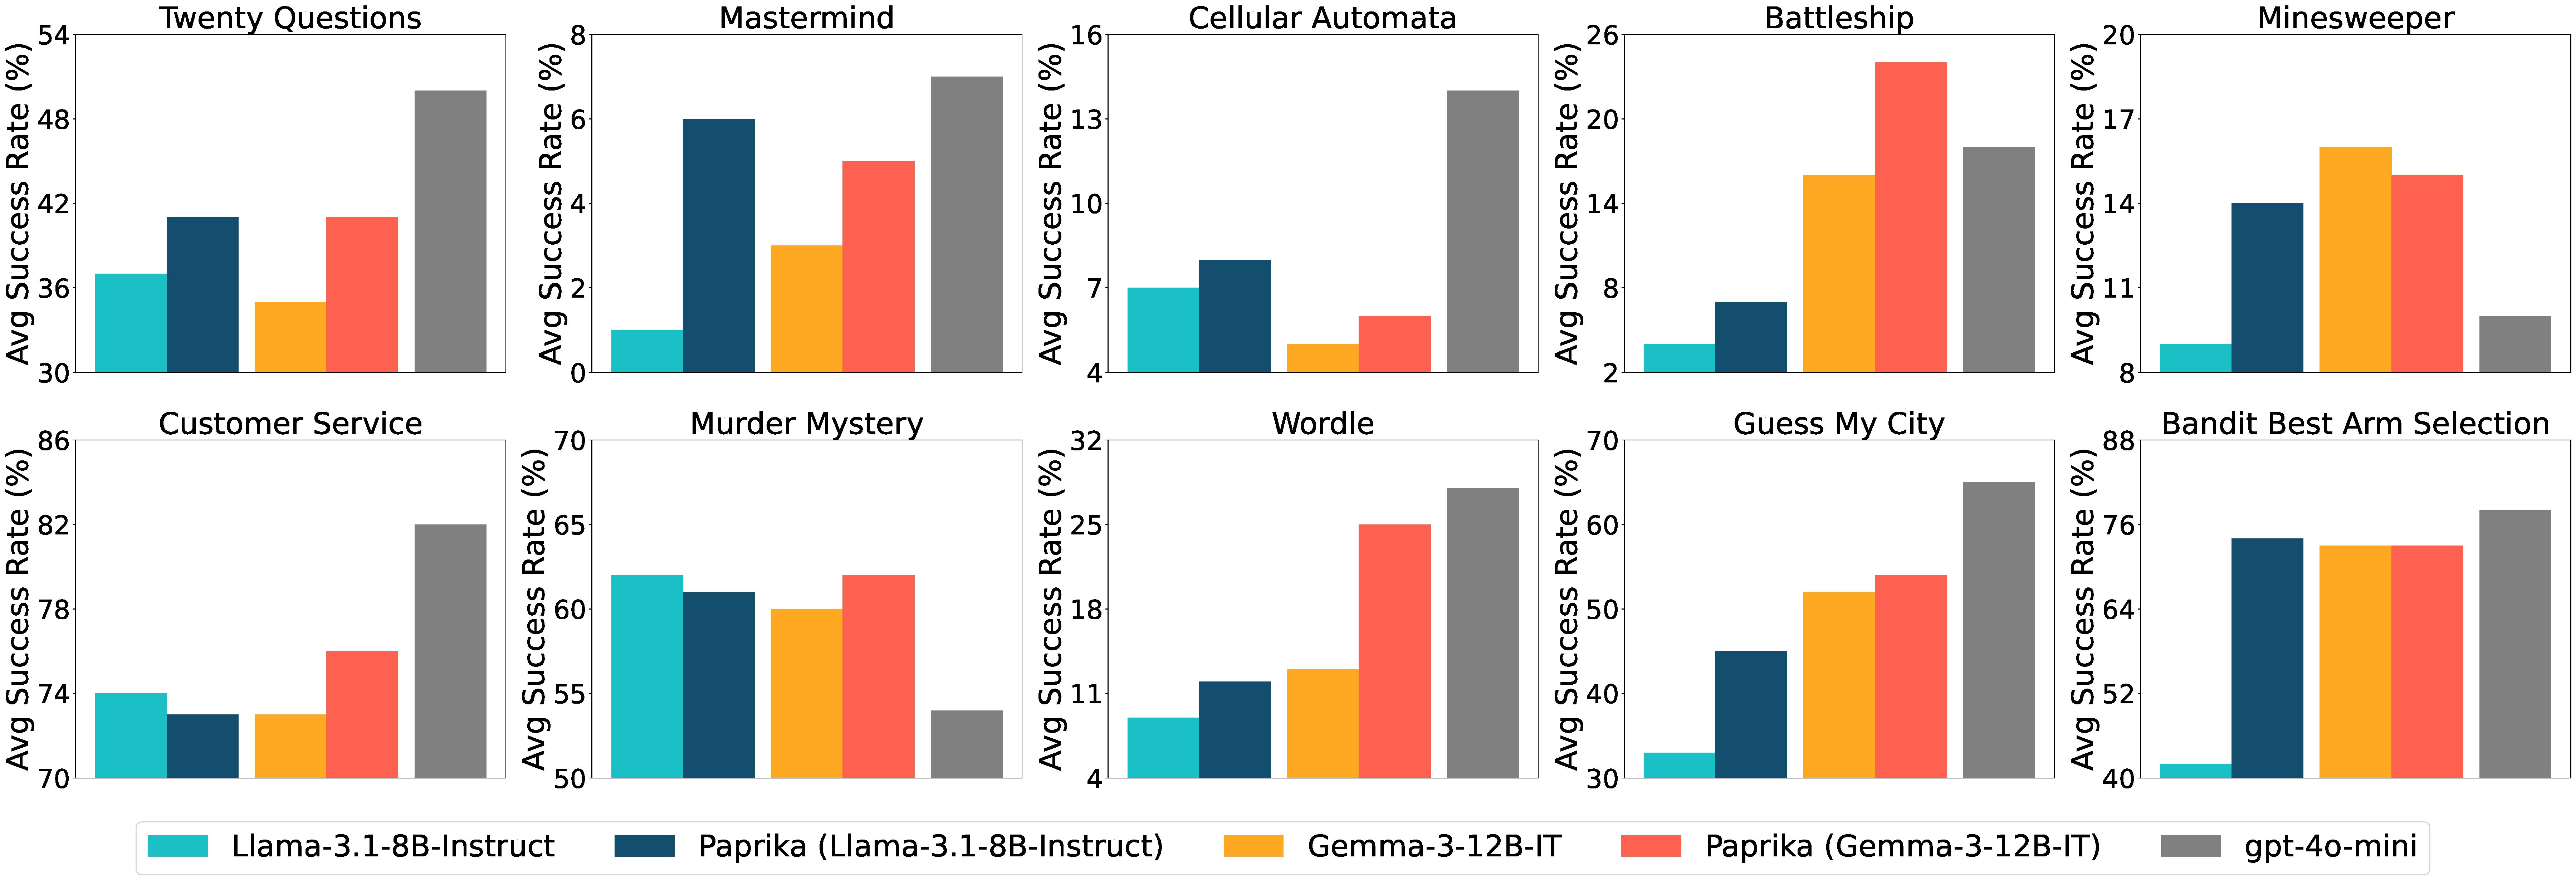
\includegraphics[width=0.99\linewidth]{figures/relative_improvement_in_success_rate.pdf}
    \vspace{-0.3cm}
    \caption{\footnotesize \textbf{(\ours{} improves success rate on a diverse range of task groups)} Average success rate on all 10 task groups at temperature 0.7. \ours{} generally improves performance of both Llama-3.1-8B-Instruct and Gemma-3-12B-IT models.}
    \label{fig:paprika_success_rate}
    \vspace{-0.2cm}
\end{figure*}

\paragraph{Sampling tasks.}Each group contains a large number of different tasks. 
Since it is infeasible to evaluate $\nu_\pi(\tau)$ for all tasks, we instead sample tasks from the group. 
This induces a scalar distribution that describes the distribution of $\nu_\pi(\tau)$ for all tasks in the group $G$.
Given a collection of $K$ groups $(G_1, \dots, G_K)$, a reasonable objective would be to maximize the learning potential of the tasks sampled. This problem can be formulated as a multi-armed bandit (MAB). Many algorithms for MAB exist; for simplicity, we choose the Upper Confidence Bound~\citep[UCB]{auer2000using}.

We conduct the task selection in a sequential manner using the original UCB algorithm, but we expect a batched variant of UCB could be used to parallelize the experience collection.
Each action corresponds to a group of tasks, and we then uniformly sample one task from the chosen group to evaluate the model performance with $C$ rollouts. These statistics are then used to update the mean estimate of that group.
After a sufficient amount of episodes are sampled, we construct the dataset and train the model with objectives in Section~\ref{sec:opt}. See Algorithm~\ref{alg:sampling} for the pseudocode.

\paragraph{Note.} An important role of $\nu_\pi$ is to make different task groups comparable. The specific selection algorithms could likely be replaced with other more sophisticated online learning methods. More importantly, recent breakthroughs such as \citet{jaech2024openai} and \citet{deepseekai2025deepseekr1incentivizingreasoningcapability} mark the beginning of applying RL to a broad range of reasoning problems. Moving forward, we anticipate a proliferation of different RL tasks for LLMs. In this emerging paradigm, a scalable meta algorithm for selecting which tasks to train on will be essential, and we believe \ours{}'s curriculum learning approach will be a promising foundation for future algorithms.




